\documentclass{article}
\usepackage[utf8]{inputenc}
\usepackage[T1]{fontenc}
\usepackage[english]{babel}
\usepackage{amsthm}
\usepackage{parskip}
\usepackage{algorithmicx}
\usepackage{amsmath}
\usepackage{algorithm}
\usepackage{algpseudocode}
\usepackage[hidelinks]{hyperref}
\newcommand\invisiblesection[1]{%
	\refstepcounter{section}%
	\addcontentsline{toc}{section}{\protect\numberline{\thesection}#1}%
	\sectionmark{#1}}
\usepackage[%
backend=biber,
style=alphabetic,
sorting=ynt,
]{biblatex}
\addbibresource{schase.bib}
\usepackage{graphicx}
\graphicspath{ {images/} }
\title{Finding Spanning Trees in Strongly Connected Graphs with Per-Vertex Degree Constraints}

\author{Samuel Chase}
\date{2018 June \linebreak\linebreak
	\small{Written under the supervision of Dr. Theresa Migler-VonDollen\linebreak\linebreak
	California Polytechnic State University, San Luis Obispo \linebreak\linebreak
	Department of Computer Science and Software Engineering \linebreak\linebreak
	© 2018 Samuel Chase}}

\begin{document}
	\maketitle
	
	\tableofcontents
	\newpage
	\section{Introduction}
	In this project, I sought to develop and prove new algorithms to create spanning trees on general graphs with per-vertex degree constraints. 
	This means that each vertex in the graph would have some additional value, a degree constraint $d$. For a spanning tree to be \textit{correct}, every vertex $v_{i}$ in the spanning tree must have a degree exactly equal to a vertex constraint $d_{i}$. This poses an additional constraint on what
	would otherwise be a trivial spanning tree problem. In this paper two proofs which inspired my studies will be discussed and analyzed, leading to my algorithm for determining a spanning tree on strongly connected graphs. It is my hope that in the future this algorithm can be modified to apply to the general case.
	
	
	
	\section{Fast vertex cover with double star graphs \\ {\small Based on "Covering by trees of small diameter" by Lov\'asz \cite{1}} }
	In his paper "Covering by trees of small diameter", Lov\'asz discusses double star graphs. A graph's diameter is the maximum number of edges to connect any two vertices in the graph. Double star graphs are graphs of diameter less than or equal to 3. A double star can be formed by adding an edge between the central nodes of any two star graphs, graphs featuring a central node with any number of edges connected only to that central node, as seen in Figure 1.
	\begin{figure}[H]
		\caption{}
		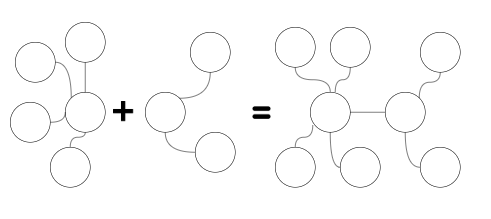
\includegraphics{Figure1}
	\end{figure}
	
	Double stars also have the interesting property of being able to cover graphs incredibly quickly. In fact, a graph of $n$ vertices be covered by a greedy algorithm taking at most $2n/3$ steps. All that is required to cover a graph with double stars is to find a maximal matching of edges, a set of edges $E$ such that no edge can be added without touching a vertex already touched by $E$. Then, add double stars centered around those edges, where the two vertices connected to the edge are individual single stars. Lov\'asz has proved that at most $2n/3$ double stars are required to cover a graph. This paper will discuss the key determinants in a maximal double-star cover, as well as provide an example of such covers on simple graphs.
	\subsection{Algorithm Overview}
	
	Lov\'asz begins by asserting that $\tau$ is the maximal number of independent vertices of $G$, a maximal set of vertices such that no two share an edge. He also states that $M$ is the maximal matching of $G$, having size $r$. $I$ is defined as the set of vertices which are not endpoints of any edges in $M$, with a size of $s$. If $n$ = $2r$ then $I$ = $\emptyset$.
	\\\\
	In section 2, it is stated that $f_{3}(g)$ is the maximum number of double stars required to cover a graph. We also know $f_{3}(g) \leq f_{2}(g)$, as even in a worst case scenario it is still impossible that double star graphs cover less efficiently than single stars. This leads Lov\'asz to know that $n-\tau \leq n-s = 2r$, or the number of vertices minus independent vertices is less than or equal to the vertices minus the vertices contained in $I$, which is equal to the number of vertices in $M$.
	\\\\
	In section 3, Lov\'asz moves on to look at $S_{i}$. For each edge $e_{i}$ in $M$, there exists $S_{i}$, a double star centered around $e_{i}$. $S_{i}$ contains the two vertices at the endpoints of $e_{i}$, and all vertices adjacent to those two vertices. $T_{i}$ is the tree of all edges containing $c_{i}$ (from $I$). We know that the set of all $S$ and $T$ covers $G$. This means $f_{3}(g) \leq r + s = n - r$, or the maximum number of double stars required to cover a graph is less than or equal to the size of $M$ plus the size of $I$. This is equal to the size of $G$ minus the size of $M$.
	\\\\
	Combining what is learned in section 4 we are able to prove Lov\'asz's theorem, that $f_{3}(g) \leq 2n/3$.
	
		\subsection{Example}
		Presented in Figure 2 is an example of graph. It may be noted that this graph itself is a double star. This reveals some of the inefficiency with this algorithm - even when a small cover (potentially even one of size 1) is available, a larger cover may be selected simply because of the nature of the greedy algorithm. It is possible for this algorithm to return multiple valid covers, depending on the sequence of selected edges.
		 \\
				\begin{figure}[H]
				\caption{}
				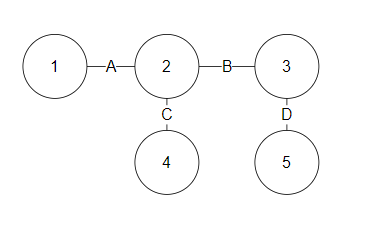
\includegraphics{Figure2}
			\end{figure}
			In Figure 2 we know that $n$ is equal to 5. Running our greedy algorithm to find a maximal matching, assume we select edges c and d. This means $M = \{c,d\}$, and therefore $r = 2$. $I$ will be all vertices not touched by $M$, therefore $I = \{1\}$ and $s$ = 1. Knowing that $f_{3}(g) \leq n-r$, we can say that the  number of double stars necessary to cover this graph is 3. An example of this maximum cover is a cover containing double stars centered around $a$, $b$, and $c$. Assuming we make the odd choice of selecting $a$ and $c$ to be the centers of our first two double stars, we notice that if we add either $b$ or $d$ we will have a full cover. Although this is something our algorithm would never provide as a $M$ (as our algorithm only seeks a maximal matching, therefore both $a$ and $c$ will never be selected), this does show a theoretical maximum size for the vertex cover. It is simply impossible to increase the maximum size, knowing that no matter which edges we choose we will cover the graph in at most 3 double stars.
			
	\section{Determining subgraphs of maximum edges on degree constrained graphs \\ {\small Based on "Another look the the degree constrained subgraph problem" by Yossi Shiloach \cite{2}}  }
	\subsection{Algorithm Overview}
	In this paper, Yossi Shiloach details an algorithm for determining subgraphs of maximum edges on a degree constrained graph $G(V,E)$. He defines
	degree constraints as a list of numbers representing the maximum degree of a vertex. However, rather than determining a spanning tree, he wishes to find an edge set, $E'$, such that $G'(V,E')$ adheres to degree constraints, while maximizing $|E'|$. The method for generating $E'$ very likely will prove useful in generalizing our own algorithm.
	\subsection{Example}
	
		\begin{figure}[H]
			\caption{}
			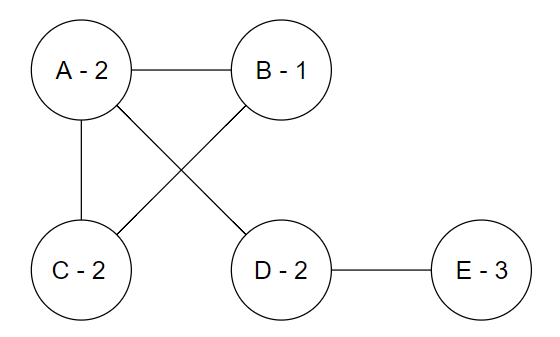
\includegraphics{Figure3}
		\end{figure}
	
	Observed in Figure 3 is a graph, with vertex labels and maximum degrees. In order to determine the maximum subgraph $G'(V,E')$ we must create graph $H$. This is done by taking every vertex, and replicating it into subvertices. A degree constraint of two produces two subvertices, a constraint of three produces three subvertices, and so on. Then, connection vertices are created, representing each edge in $G$. Therefore, as depicted in Figure 4,there will be a vertex created for $A$->$B$ and a vertex for $B$->$A$. $A$->$B$ will connect to every subvertex of $A$, while  $B$->$A$ will connect to every subvertex of $B$. Then $A$->$B$ will be connected to  $B$->$A$. This will be done for every edge in $G$, to yield a new graph $H$.
	
	\begin{figure}[H]
		\caption{}
		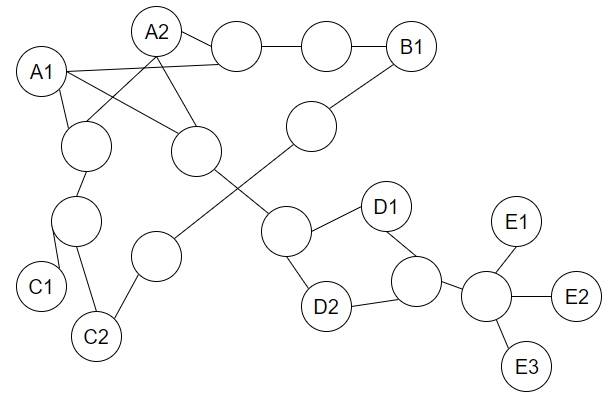
\includegraphics{Figure4}
	\end{figure}

	Following this, a maximum matching must be drawn on $H$, such as the one depicted in Figure 5. Bolded edges are in the matching.
	
		\begin{figure}[H]
		\caption{}
		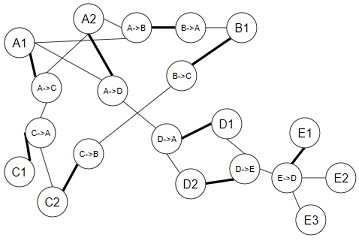
\includegraphics{Figure5}
	\end{figure}
		 		\vbox{%
	Then, one must look at the edges between the unlabeled connector vertices. An edge will be in $E'$, unless the edge between the connectors is in the matching, as in the $A$ <-> $B$ connector. $G'$ is shown below in Figure 6. It can be verified that $G'$ does not violate any degree constraints and contains a maximum valid edge set $E'$.
}
	\begin{figure}[H]
		\caption{}
		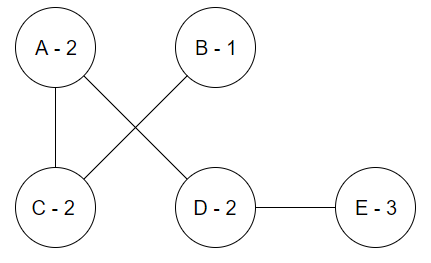
\includegraphics{Figure6}
	\end{figure}

	One might notice that on certain graphs there are more than one maximum matching, which may yield different $G'$s. This is expected, as in many cases there are multiple $G'$s, both with maximum $|E'|$. In these cases all possible $G'$s returned by the algorithm are valid.

	\newtheorem{theorem}{Theorem}
	\section{Spanning trees in connected graphs with per-vertex degree constraints}
	\subsection{Algorithm Overview}
	Assume that we wish to create a spanning tree for a graph. Correct algorithms for solving this problem have been proven by Kruskal and other
	mathematicians, however, in this case, we wish to consider per-vertex degree constraints. Assume that in the graph every vertex, $v_{i}$, has some degree constraint $d_{i}$,
	where for a spanning tree to be valid $v_{i}$ must be equal to $d_{i}$ for all $v_{i} \in V$
	\\\\\\\\\\
	
	An algorithm for solving this problem can be seen below:
	\\

		\begin{algorithm}[H]
		\caption{Creating a spanning tree on a strongly connected graph with per-vertex degree constraints}
		\begin{algorithmic}[1]
			\State Graph $G(V,E)$ with a total degree of $2(|V|-1)$
			\State T = $\emptyset$
			\State T += ($v1$,$v2$) where $v1$ is the vertex of largest degree in V, and $v2$ is the vertex of second largest degree. Decrement the degree of $v1$ and $v2$
			\While{There exits a vertex in $V$ and $T$ with a degree $>$ 0 }
			\State \parbox[t]{\dimexpr\linewidth-\algorithmicindent}{T+= ($t$,$v$) where $t$ is the vertex of largest degree in $t$, and $v$ is the largest vertex in $V$\textbackslash$T$\strut}
			\EndWhile
		\end{algorithmic}
	\newpage
	\end{algorithm}
	\subsection{Proof of Correctness}
	\begin{theorem}
		Given a strongly connected graph $G(E,V)$ with total vertex degree constraint of $2(|V|-1)$ algorithm 1 will return a correct spanning tree.
	\end{theorem}

	\begin{proof}
		Allow the algorithm to run until step 3, producing tree $T$. $G$ will have a total degree constraint of $2(|V|-1)-2$, accounting for the single edge in T. Therefore, $G$ has a total degree constraint of $2(|V|-2)$, and needs to connect $|V|-2$ vertices to $T$. Thus it will be possible to complete the spanning tree, as the total degree constraint of $G$ is equal to twice the number of vertices not in $T$, and $T$ will either have a total degree constraint $\geq$ 1, or be $G$. 
		\\
		\\
		Now, assume $T$ has grown to size k vertices correctly, where $T$ has a total degree constraint large enough to complete the spanning of the graph. $T$ will now select the next untouched vertex of maximum degree. There are 3 cases for this vertex:
		

		\setlength\parindent{12pt} 
		Case 1) The next vertex selected has a degree = 1 \par
		\setlength\parindent{24pt}\hangindent=24pt 
		In this case, if the largest vertex remaining has a degree constraint of 1 then all vertices not in $T$, called $U$, must
		have a degree constraint of 1. Thus $T$ must have a total remaining vertex constraint of $|V \setminus U|$, which is equal to  $|U|$. Therefore, as there are $|U|$ vertices not in $T$ and $T$ has a total degree constraint of $|U|$, we know the degree constraint will not be violated, as each connection from $T$ to $U$ lowers the total degree constraint by one.  Thus $T$ will be able to complete the spanning tree.
		\par



		\setlength\parindent{12pt}
		Case 2) The next vertex selected has a degree $>$ 1\par
		\setlength\parindent{24pt}\hangindent=24pt 
		Adding this vertex to $T$ will increase $T$'s total degree constraint by some value $>$ 1, and then decrease $T$'s total degree constraint by 2.
		Therefore the change in $T$ cannot be less than zero, and $T$ will not be decreased, so $T$ will be able to complete the spanning tree.
		\par
	
		\vbox{%
		\setlength\parindent{12pt}
		Case 3) No new vertex can be selected\par
		\setlength\parindent{24pt}\hangindent=24pt 
		If no new vertex can be selected this means every vertex in $G$ is in $T$. Thus the spanning tree will be completed.
		\par
	}
		
		\setlength\parindent{0pt}\hangindent=0pt
		Therefore it is clear that $T$ will not violate degree constraints at every step of the algorithm, and the algorithm will proceed to completion.
		
	\end{proof}	
	\section{Conclusion}
	
	The goal of this project was to determine an algorithm to produce spanning trees on graphs with per-vertex degree constraints. I was able to produce an algorithm and proof, which work on strongly connected graphs. I hope that perhaps future researchers might modify my algorithm, and potentially utilize the techniques of Yossi Shiloach, to solve the general case.
	
	\newpage
\invisiblesection{References}
	\begin{thebibliography}{9}
		\bibitem{lovasz}
		Lovász, L. (1968). On covering of graphs (P. Erdos \& G. Katona, Eds.). Theory of Graphs, 234-235. 
		
		\bibitem{shiloach}
		Shiloach, Y. (1981). Another look at the degree constrained subgraph problem. Inf. Process. Lett., 12, 89-90.
		
	\end{thebibliography}
	
\end{document}
